% !TeX root = ./moreau_lt.tex
\documentclass{beamer}

\usepackage{beamer_tom}
\graphicspath{{./images/}}

\def\biblio{
    \nobibliography{../../library}
    \def\biblio{}
}

\institute{INRIA Saclay}
\author{Thomas Moreau}
\title{
    Distributed Optimization for\\Convolutional Dictionary Learning}

\date{
    May 29, 2018
}

\setbeamertemplate{title page}[header]
\def\extraLogo{}

\newcommand{\techterm}[2][1-]{
    \column{\widthof{\bf #2}}
    \visible<#1>{
    \centering
    \begin{beamercolorbox}[rounded=true, shadow=true]{title}
        \bf \phantom{g}\hskip-\skipg #2
    \end{beamercolorbox}
    }
}

\begin{document}

    \frame[t]{
        \titlepage
        \centering%
        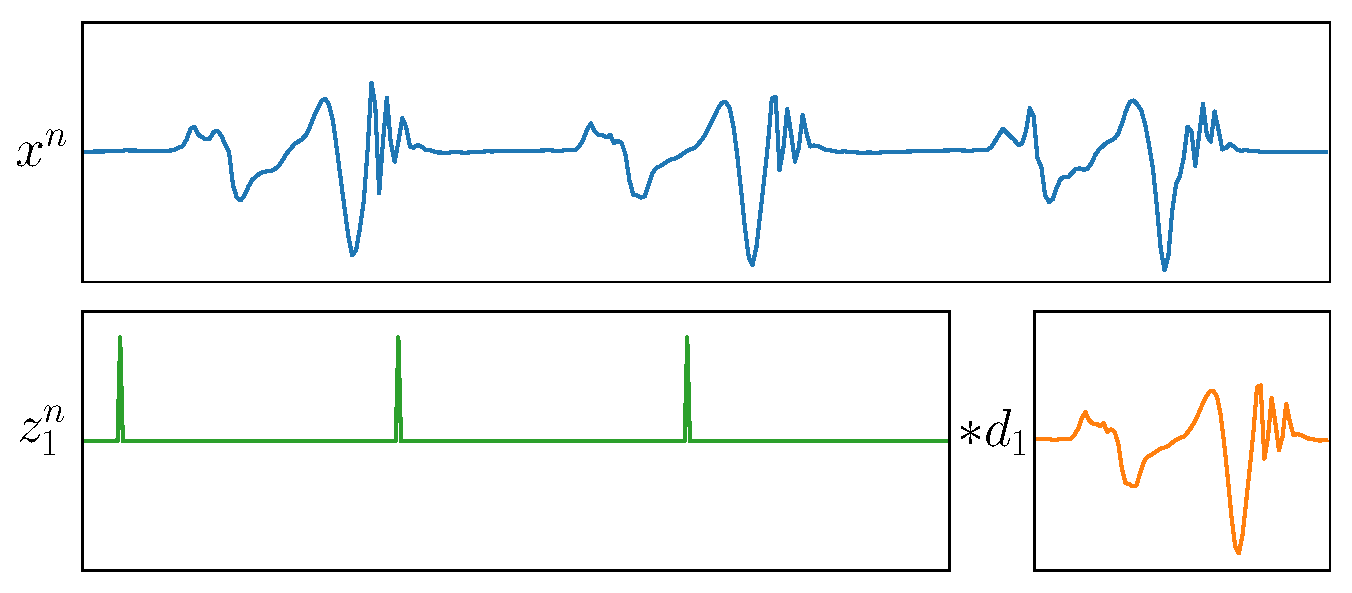
\includegraphics[width=\textwidth]{intro_csc_5}%
        \vskip-.5em%
        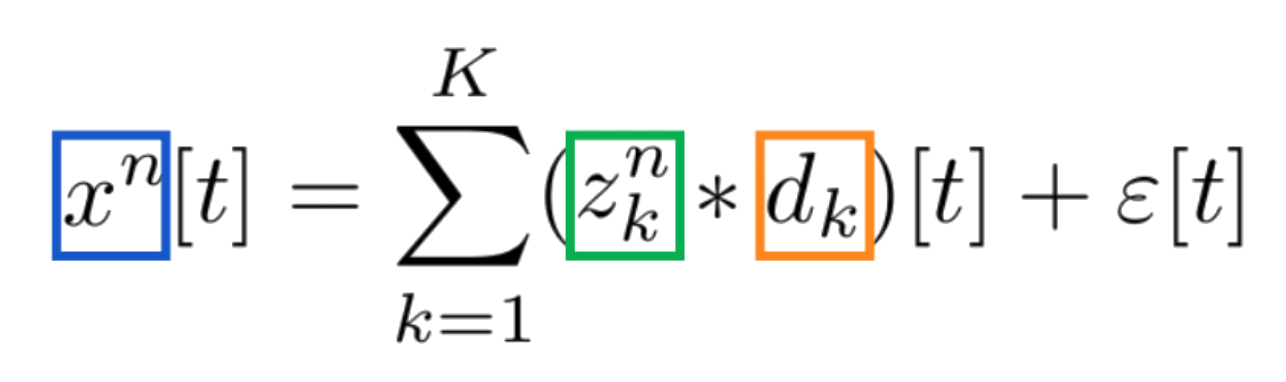
\includegraphics[width=.6\textwidth]{csc_explain_eq_color}%
    }

    \frame[t]{
        \frametitle{Optimization for CDL}

        {\bf Parameter estimation:} Bi-convex optimization problem.
        \[
            \argmin_{z^n, \|d_k\|_2 \le 1}\sum_{n=1}^N \underbrace{\|x^n - \sum_{k=1}^K z_k^n * d_k\|_2^2}_{f(z_k, d_k)}
                         + \lambda \|z^n\|_1
        \]


        {Solved with block coordinate descent \emph{a.k.a.} Alternate minimization.\\[1.5em]}
        {
        \centering
        \bgroup
        \def\arraystretch{1.5}%
        \begin{tabular}{| c || c |}
            \hline
            $z$-step  & $d$-step\\\hline\hline
            Coordinate descent & Projected Gradient descent\\\hline
            Local computation in time & Global computation in time\\\hline
            Parallel updates & Parallel pre-computation\\\hline

        \end{tabular}\\
        \egroup
        }


    }

\begin{frame}[t]{Distributed convolutional sparse coding}

    {\bf $z$-step:} Estimating $z$ for a fixed dictionary $d$ with CD
    \vskip-.5em
    \[
        \argmin_{z_k} \| x - \sum_{k=1}^K z_k * d_k\|_2^2
            + \lambda\sum_{k=1}^K\|z_k\|_1
    \]
    {
        \centering
        \inputTikZ{.7}{DICOD}\\[.5em]
    }

    \only<3->{
        {\vskip-1em\bf Distributed coordinate descent\\[.5em]}
        \begin{columns}[c]
        \column{.5ex}
        \techterm[3-]{\small Asynchronous}
        \column{.5ex}
        \techterm[4-]{\small Local Communications}
        \column{.5ex}
        \techterm[5]{\small Soft-Lock}
        \column{.5ex}
        \end{columns}
    }%
\end{frame}

\frame[t]{
    \frametitle{Updating the dictionary in the distributed setup}

    {\bf $d$-step:} updating $d$ for fixed activations $z$ with PGD\\[-.5em]
    \[
        \argmin_{\|d_k\|_2 = 1} \sum_{n=1}^N
            \| x^n - \sum_{l=1}^K z_l^n * d_l\|_2^2
    \]
    {\textbf{Bottleneck:} Gradient computation in $\bO{KT\log T}$\\[-1.5em]}
    \begin{eqnarray*}
        \nabla_{d_k}f(d_k, z_k) & = & z_k^\Lsh * (x - \sum_{k=1}^K z_k * d_k)\\
                                & = & \underbrace{z_k^\Lsh * x}_{\phi_k} - \sum_{l=1}^K \underbrace{z_l^\Lsh * z_l}_{\psi_{k, l}} * d_l)
    \end{eqnarray*}
    By pre-computing $\phi_k$ and $\psi_{k, l}$, the gradient computation in $\bO{KL\log L}$~.\\[1em]
    Use the distributed setting to compute these constants.

}

\frame{
    \frametitle{Take Home Message}

    \textbf{Easy Distributed Computation:}\\[1em]
    {\centering Workers do mostly independent work.\\[2em]}
    \textbf{Finite support convolution:}\\[1em]
    {\centering Far enough coefficients are weakly dependent.\\[2em]}

    \begin{columns}[c]
        \column{.45\textwidth}
        \begin{beamercolorbox}[rounded=true, shadow=true,wd=\textwidth]{title}
            \centering \bf \phantom{g}\hskip-\skipg
            Local computations can be\\ done asynchronously
        \end{beamercolorbox}
        \column{.45\textwidth}
        \begin{beamercolorbox}[rounded=true, shadow=true, wd=\textwidth]{title}
            \centering \bf \phantom{g}\hskip-\skipg
            Global computations are\\ synchronous operations.
        \end{beamercolorbox}
    \end{columns}
    \vskip2em
    \centering \large $\neq$ from ADMM/ISTA frameworks with global computations.


}
\end{document}